\noindent

\includegraphics[height=1.25cm]{images/pictograms/replication}

\includegraphics[height=1.25cm]{images/pictograms/benchmark}

\includegraphics[height=1.25cm]{images/pictograms/under_construction}

\includegraphics[height=1.25cm]{images/pictograms/FEM}
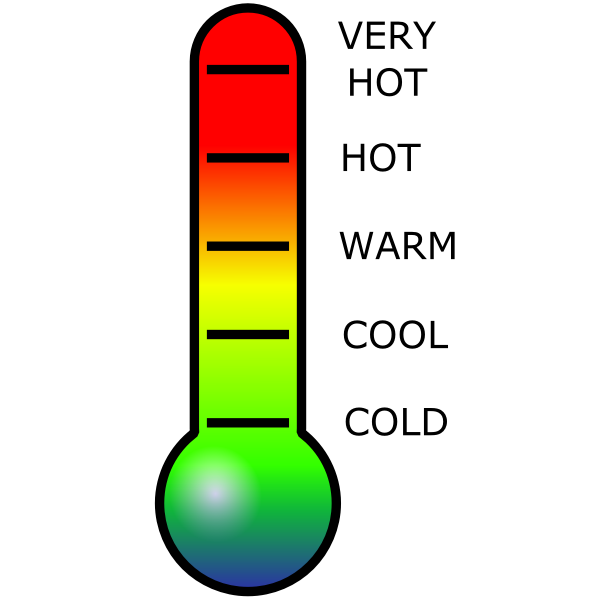
\includegraphics[height=1.25cm]{images/pictograms/temperature}

\includegraphics[height=1.25cm]{images/pictograms/paraview}

%%%%%%%%%%%%%%%%%%%%%%%%%%%%%%%%%%%%%%%%%%%%%%%%%%%%%%%%%%%%%%%%%%%%%%%%%%%%%%%%%%%%%%%%%%%%%%%%%%%

\begin{flushright} {\tiny {\color{gray} python\_codes/fieldstone\_173/text.tex}} \end{flushright}

%\lstinputlisting[language=bash,basicstyle=\small]{python_codes/template_keywords.key}

\par\noindent\rule{\textwidth}{0.4pt}

\begin{center}
\inpython
{\small Code: \url{https://github.com/cedrict/fieldstone/tree/master/python_codes/fieldstone_173}}
\end{center}

\par\noindent\rule{\textwidth}{0.4pt}

{\sl This stone was developed in collaboration with Donald Duck}. \index{contributors}{D. Duck}

\par\noindent\rule{\textwidth}{0.4pt}

Last revision: May. 23th, 2025.

\par\noindent\rule{\textwidth}{0.4pt}

%%%%%%%%%%%%%%%%%%%%%%%%%%%%%%%%%%%%%%%%%%%%%%%%%%%%%%%%%%%%%%%%%%%%%%%%%%%%%%%%%%%%%%%%%%%%%%%%%%%


\section*{Setup}

The domain is the unit square. 
The 2d steady state heat equation (with heat source) is solved, with $\rho=C_p=k=1$:
\[
\frac{\partial^2 T}{\partial x^2} + \frac{\partial^2 T}{\partial y^2} + S(x,y) = 0
\]
with $S(x,y)=-10$. 
The exact solution is 
\[
T(x,y)=(2x+y)^2
\]
since 
\[
\frac{\partial^2 T}{\partial x^2} + \frac{\partial^2 T}{\partial y^2}
= 2\cdot 2 \cdot 2 + 2 \cdot 1 \cdot 1 = 10
\]
The heat flux vector is then given by\footnote{the heat conductivity is equal to 1}
\[
\vec{q} = - \vec{\nabla} T = -2(2x+y) (2 \vec{e}_x + \vec{e}_y)
\]


We now turn to Figure 2 of the paper:
\begin{center}
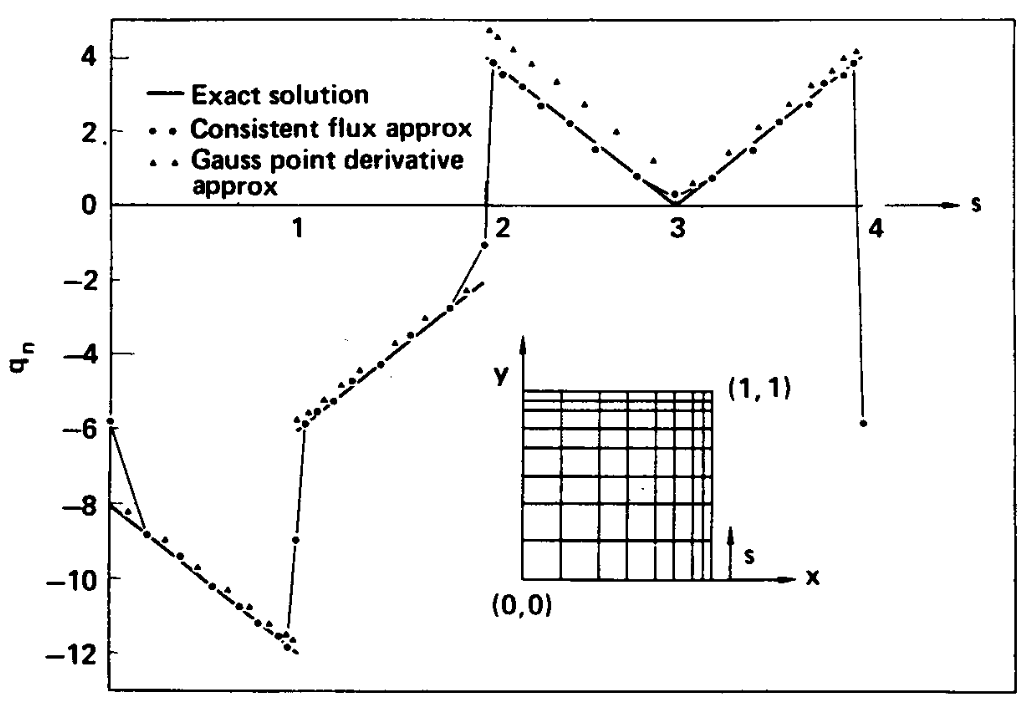
\includegraphics[width=7cm]{python_codes/fieldstone_173/images/grls87a}
\end{center}

We learn from it that the mesh counts $8\times 8$ elements with a gradual size change in space.
This is implemented as follows:
\begin{lstlisting}
for i in range(0,NV):
    x[i]=x[i]**0.66
    y[i]=y[i]**0.66
\end{lstlisting}

The mesh then looks like this:

\begin{center}
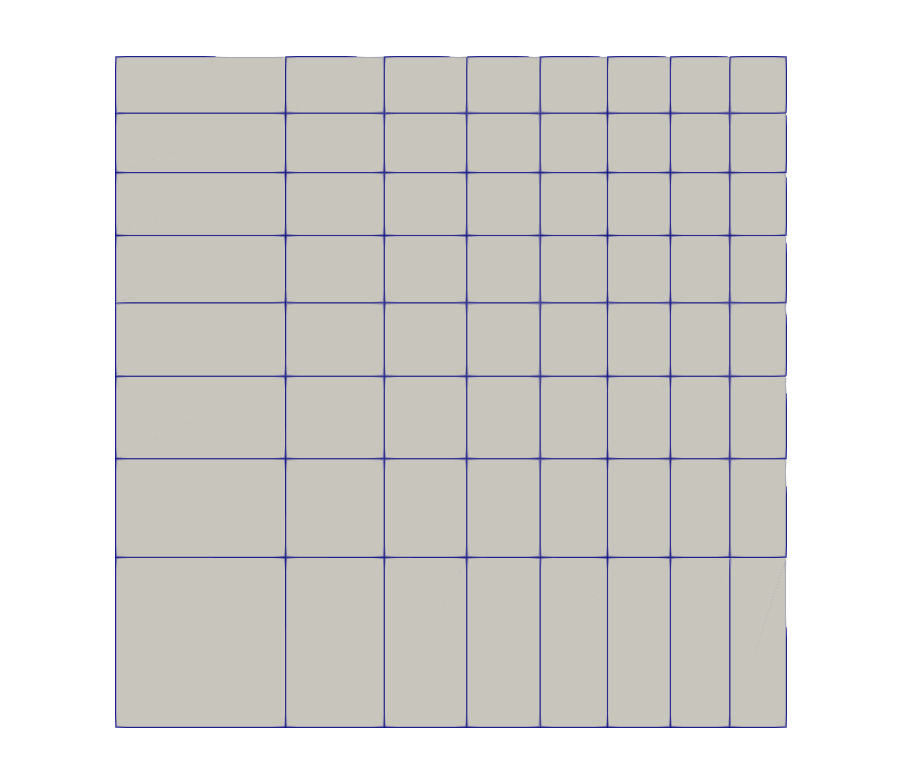
\includegraphics[width=7cm]{python_codes/fieldstone_173/images/mesh8x8}
\end{center}
This is not identical to the article but sufficiently close.


We then solve the equation on this mesh with $Q_1$ elements:

\begin{center}
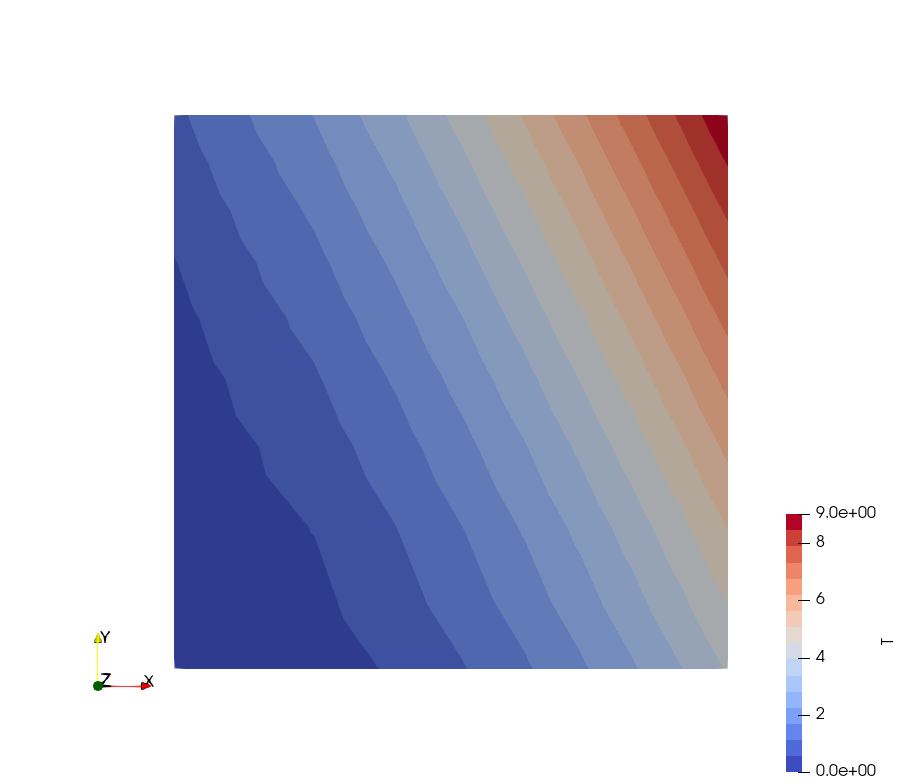
\includegraphics[width=5.7cm]{python_codes/fieldstone_173/results/T}
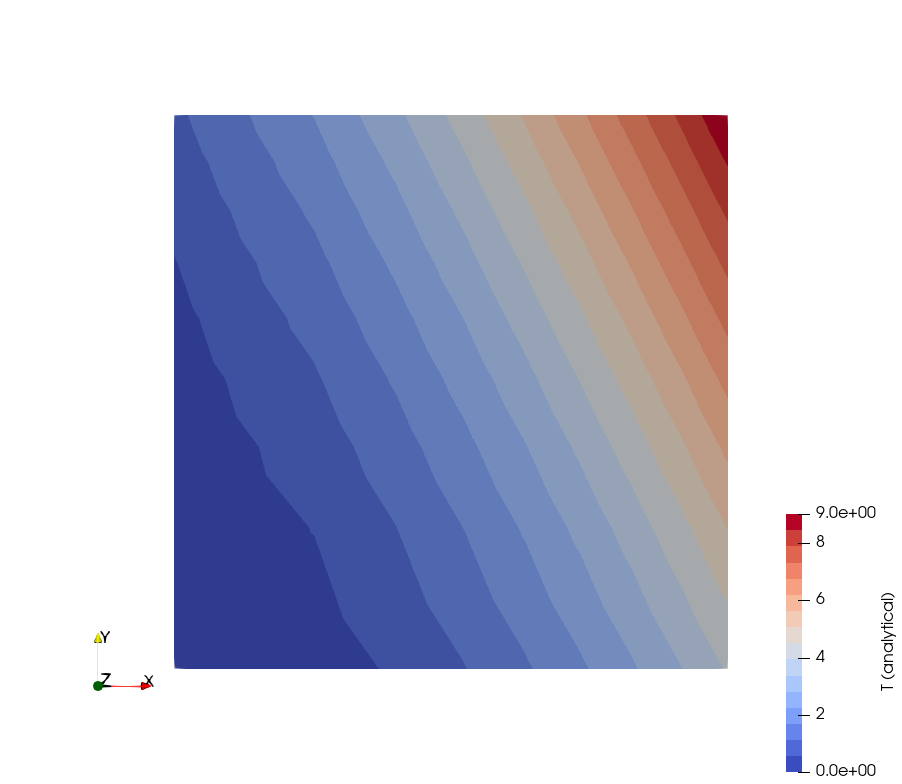
\includegraphics[width=5.7cm]{python_codes/fieldstone_173/results/T_analytical}
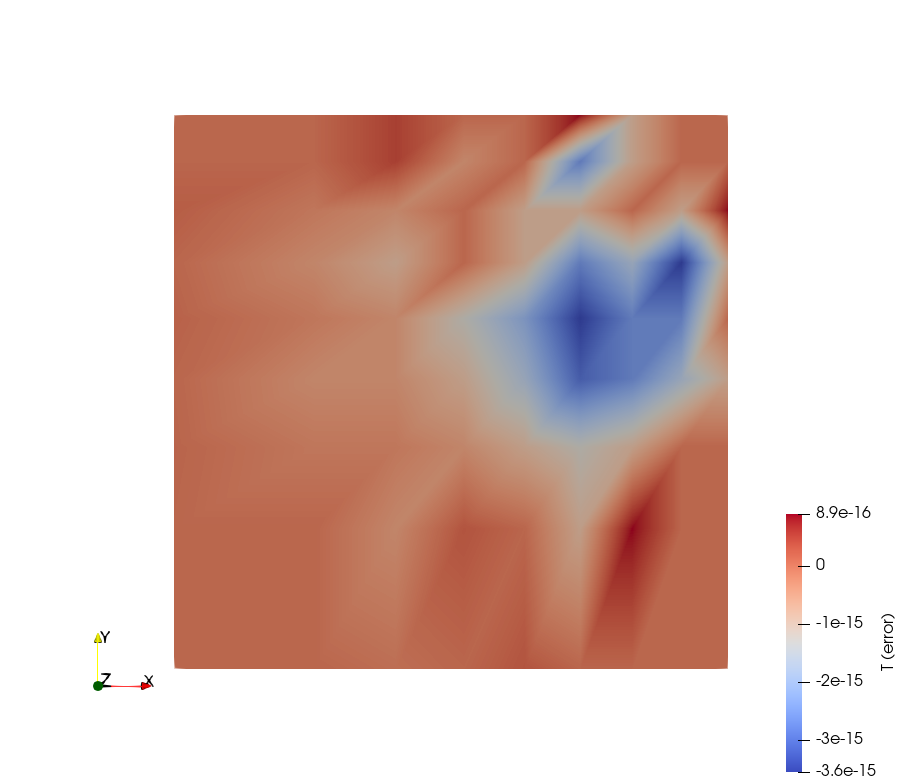
\includegraphics[width=5.7cm]{python_codes/fieldstone_173/results/T_error}\\
{\captionfont Temperature in the domain on stretched $8\times 8$ mesh. 
Left: computed; Middle: analytical; Right: error.}
\end{center}

We find that the calculated temperature is machine precision accurate.




%==============================================================================
\section*{Computing boundary normals}

Given the geometry of the domain, computing the normal to the boundary 
should not pose much problem. However, we need the normal vector at the nodes,
including the corner nodes. An inescapable question arises: 
what is the normal vector at the corners?

One option is to state that the problem is ill-posed and that the normal to a
singular point does not exist.

Another option is to look at the geometry of the domain (a rectangle), see that 
the corners then belong to two faces with normals orthogonal to each other 
and then set the normal vector to the average of the adjacent face normals.
For example the normal vector at point $(1,1)$ would then be $\vec{n}=(1,1)/\sqrt{2}$.

Finally, the last option is to follow the approach 
explained in \textcite{ensg82}: 
the normal vector at a node $i$ can be computed using the basis function derivatives:
\begin{eqnarray}
n_{x,i} &=& \frac{1}{n_i}\int_\Omega \frac{\partial \bN_i}{\partial x} dV \nn\\
n_{y,i} &=& \frac{1}{n_i}\int_\Omega \frac{\partial \bN_i}{\partial y} dV \nn
\end{eqnarray}
with 
\[
n_i = \left[
\left(\int_\Omega \frac{\partial \bN_i}{\partial x} dV\right)^2 +
\left(\int_\Omega \frac{\partial \bN_i}{\partial y} dV\right)^2 
\right]^{1/2}
\]

The integral over $\Omega$ is actually cheap: the nodes in question are on the boundary, 
and their basis functions have a compact support (on the boundary a node belongs to at 
most 2 elements) so that the code is as follows:

\begin{lstlisting}
nx=np.zeros(NV,dtype=np.float64) 
ny=np.zeros(NV,dtype=np.float64) 
jcb=np.zeros((ndim,ndim),dtype=np.float64)

for iel in range(0,nel):
    if surface_element[iel]: 
       for iq in range(0,nqperdim):
           for jq in range(0,nqperdim):

               rq=qcoords[iq]
               sq=qcoords[jq]
               weightq=qweights[iq]*qweights[jq]
               dNNNTdr=dNNTdr(rq,sq,order)
               dNNNTds=dNNTds(rq,sq,order)
               jcb[0,0]=np.dot(dNNNTdr[:],x[icon[:,iel]])
               jcb[0,1]=np.dot(dNNNTdr[:],y[icon[:,iel]])
               jcb[1,0]=np.dot(dNNNTds[:],x[icon[:,iel]])
               jcb[1,1]=np.dot(dNNNTds[:],y[icon[:,iel]])
               jcob = np.linalg.det(jcb)
               jcbi=np.linalg.inv(jcb)
               dNNNTdx=jcbi[0,0]*dNNNTdr[:]+jcbi[0,1]*dNNNTds[:]
               dNNNTdy=jcbi[1,0]*dNNNTdr[:]+jcbi[1,1]*dNNNTds[:]
               for k in range(0,m):
                   if boundary_node[icon[k,iel]]:
                      nx[icon[k,iel]]+=dNNNTdx[k]*jcob*weightq
                      ny[icon[k,iel]]+=dNNNTdy[k]*jcob*weightq
\end{lstlisting}
which is then followed by a normalisation:
\begin{lstlisting}
for i in range(0,NV):
    if boundary_node[i]:
       norm=np.sqrt(nx[i]**2+ny[i]**2)
       nx[i]/=norm
       ny[i]/=norm
\end{lstlisting}

In this case the normal vectors are as follows:
\begin{center}
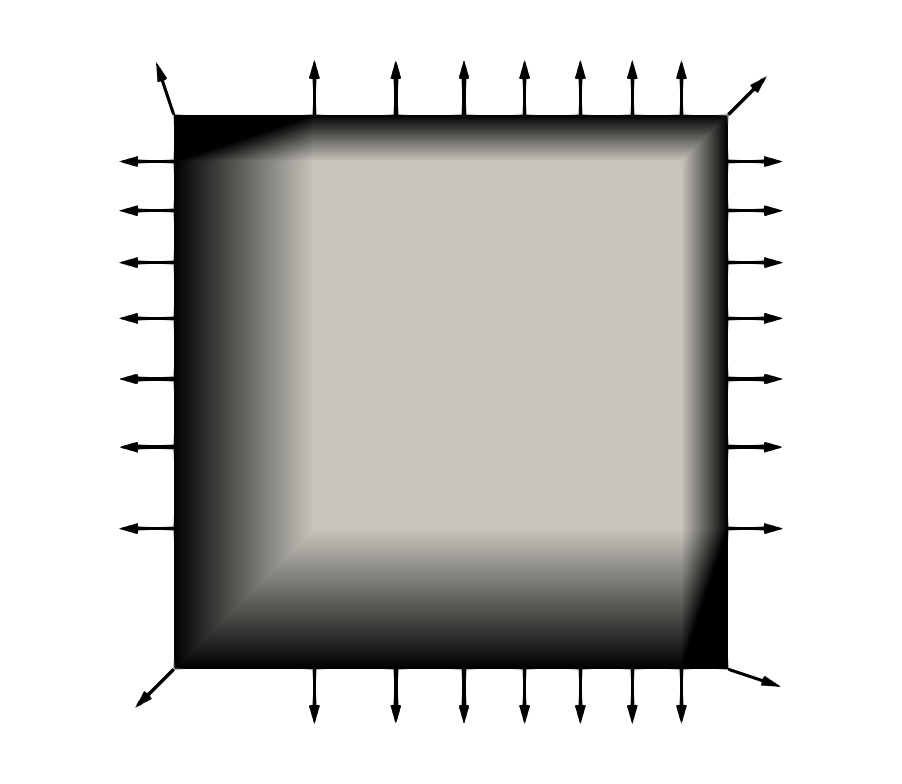
\includegraphics[width=5.7cm]{python_codes/fieldstone_173/results/normals}
\end{center}
We see that the vectors at the corners are not 'at $45$ degrees' if the element is not square.


%==============================================================================
\section*{Computing the nodal heat flux everywhere - method 1}

We apply here a standard technique: the derivatives of the temperature 
are computed at each corner of the element by means of the basis functions
and then averaged out on the nodes.

\begin{lstlisting}
    qx=np.zeros(NV,dtype=np.float64) 
    qy=np.zeros(NV,dtype=np.float64) 
    qn=np.zeros(NV,dtype=np.float64) 
    cc=np.zeros(NV,dtype=np.float64) 
    for iel in range(0,nel):
        for k in range(0,m):
            rq=rnodes[k]
            sq=snodes[k]
            inode=icon[k,iel]
            cc[inode]+=1
            dNNNTdr=dNNTdr(rq,sq,order)
            dNNNTds=dNNTds(rq,sq,order)
            jcb=np.zeros((ndim,ndim),dtype=np.float64)
            jcb[0,0]=np.sum(dNNNTdr[:]*x[icon[:,iel]])
            jcb[0,1]=np.sum(dNNNTdr[:]*y[icon[:,iel]])
            jcb[1,0]=np.sum(dNNNTds[:]*x[icon[:,iel]])
            jcb[1,1]=np.sum(dNNNTds[:]*y[icon[:,iel]])
            jcbi=np.linalg.inv(jcb)
            dNNNTdx[:]=jcbi[0,0]*dNNNTdr[:]+jcbi[0,1]*dNNNTds[:]
            dNNNTdy[:]=jcbi[1,0]*dNNNTdr[:]+jcbi[1,1]*dNNNTds[:]
            qx[inode]-=np.sum(dNNNTdx[:]*T[icon[:,iel]])
            qy[inode]-=np.sum(dNNNTdy[:]*T[icon[:,iel]])
        #end for
    #end for
    qx/=cc
    qy/=cc
    qn[:]=qx[:]*nx[:]+qy[:]*ny[:]
\end{lstlisting}

We find that this technique yields an accurate heat flux inside the domain 
but not so much on the boundary:

\begin{center}
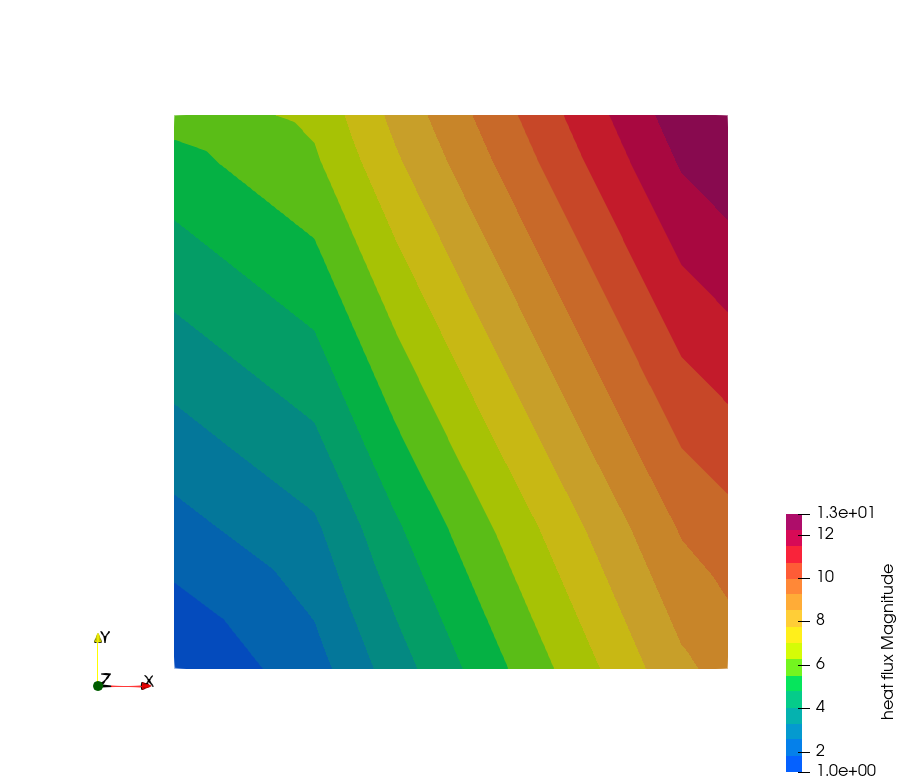
\includegraphics[width=5.7cm]{python_codes/fieldstone_173/results/q8}
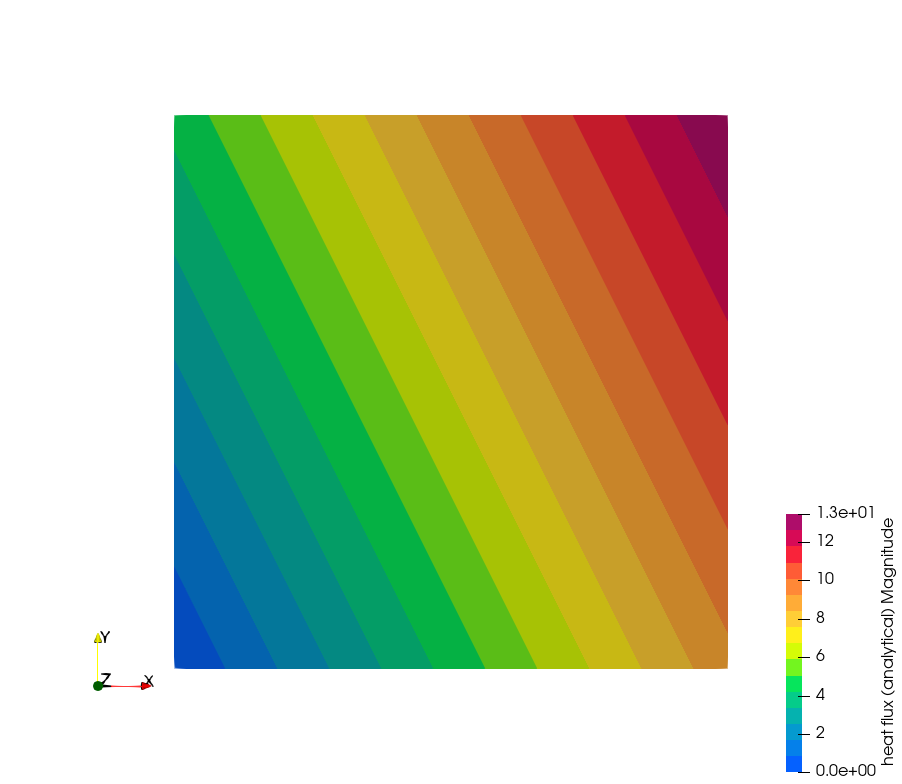
\includegraphics[width=5.7cm]{python_codes/fieldstone_173/results/q8_analytical}
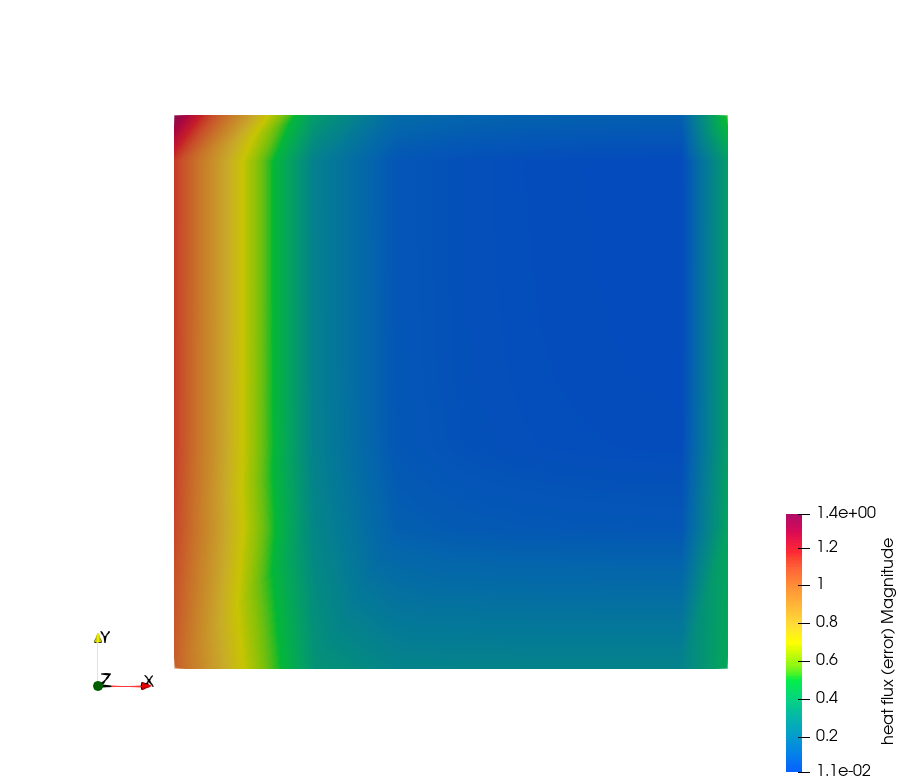
\includegraphics[width=5.7cm]{python_codes/fieldstone_173/results/q8_error}\\
{\captionfont Temperature in the domain on $8 \times 8$ mesh.}
\end{center}

We can also compute the heat flux on a higher resolution mesh:
\begin{center}
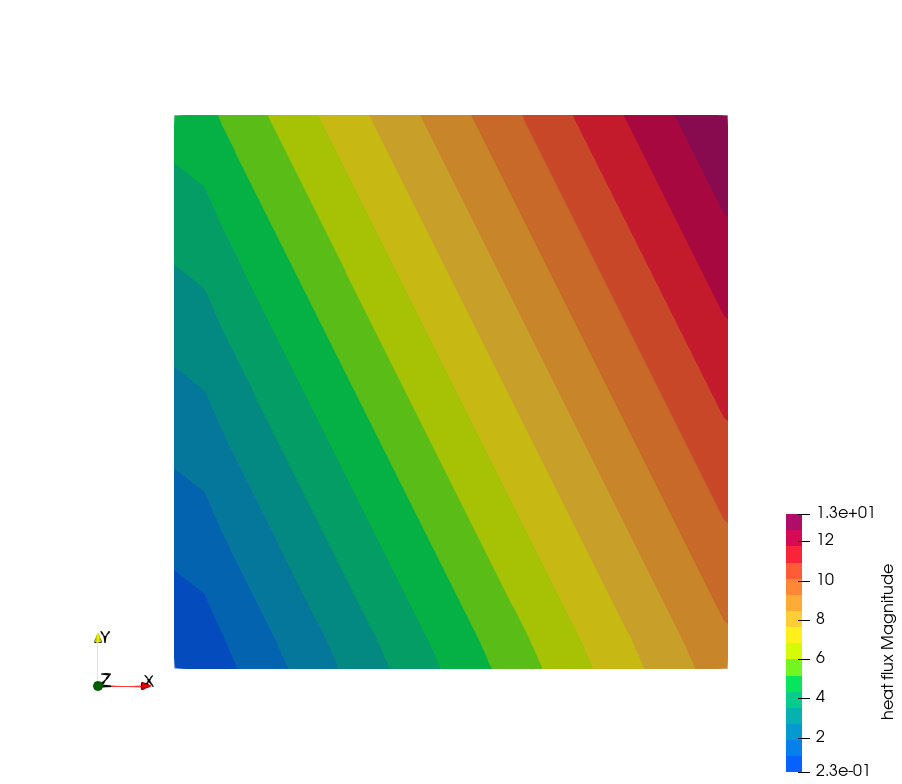
\includegraphics[width=5.7cm]{python_codes/fieldstone_173/results/q80}
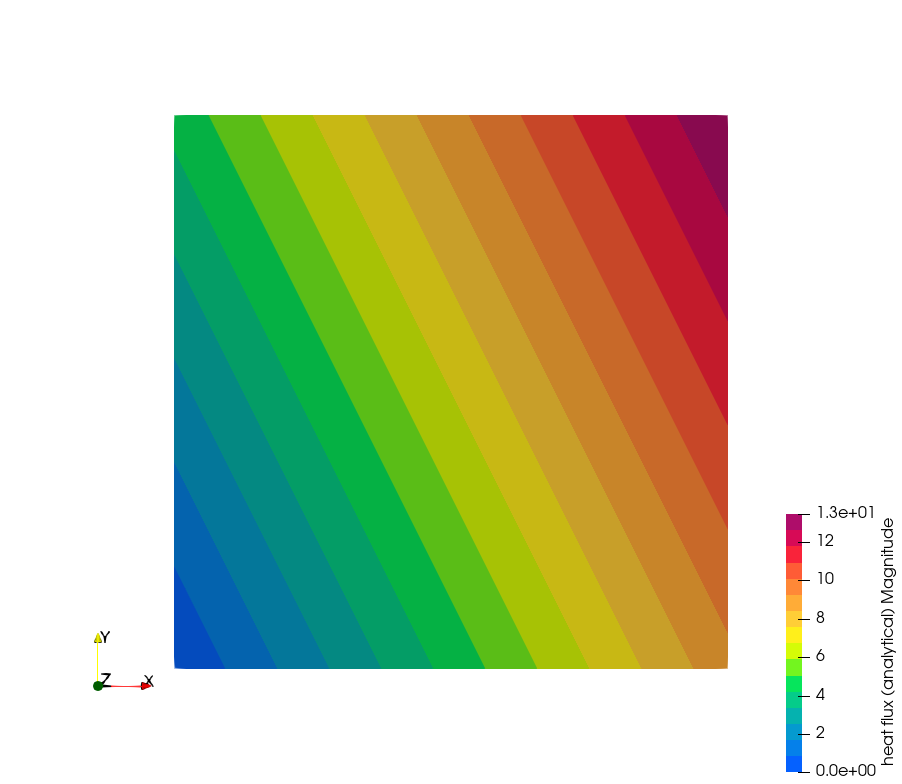
\includegraphics[width=5.7cm]{python_codes/fieldstone_173/results/q80_analytical}
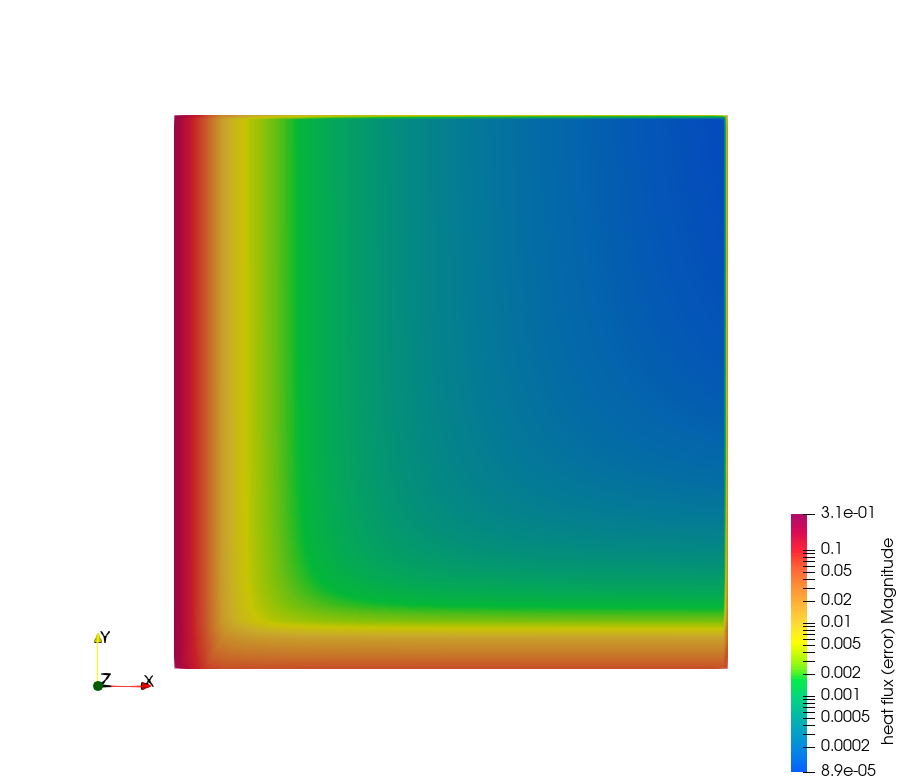
\includegraphics[width=5.7cm]{python_codes/fieldstone_173/results/q80_error}\\
{\captionfont Temperature in the domain on $80 \times 80$ mesh.}
\end{center}

In both cases we see that the heat flux is not accurate on the boundary.
As in \textcite{grls87} we can plot the normal heat flux, i.e. $q_n=\vec{q}\cdot \vec{n}$
along the boundary starting a the SE corner, moving to NE, then NW, then SW back to SE:

\begin{center}
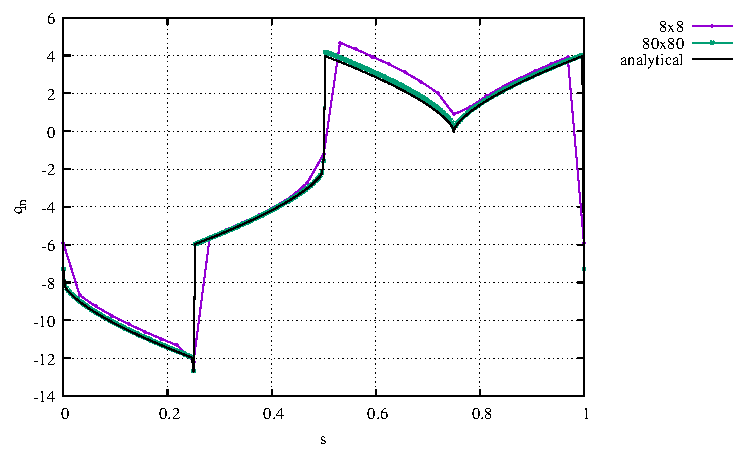
\includegraphics[width=8.5cm]{python_codes/fieldstone_173/results/heat_flux_boundary.pdf}
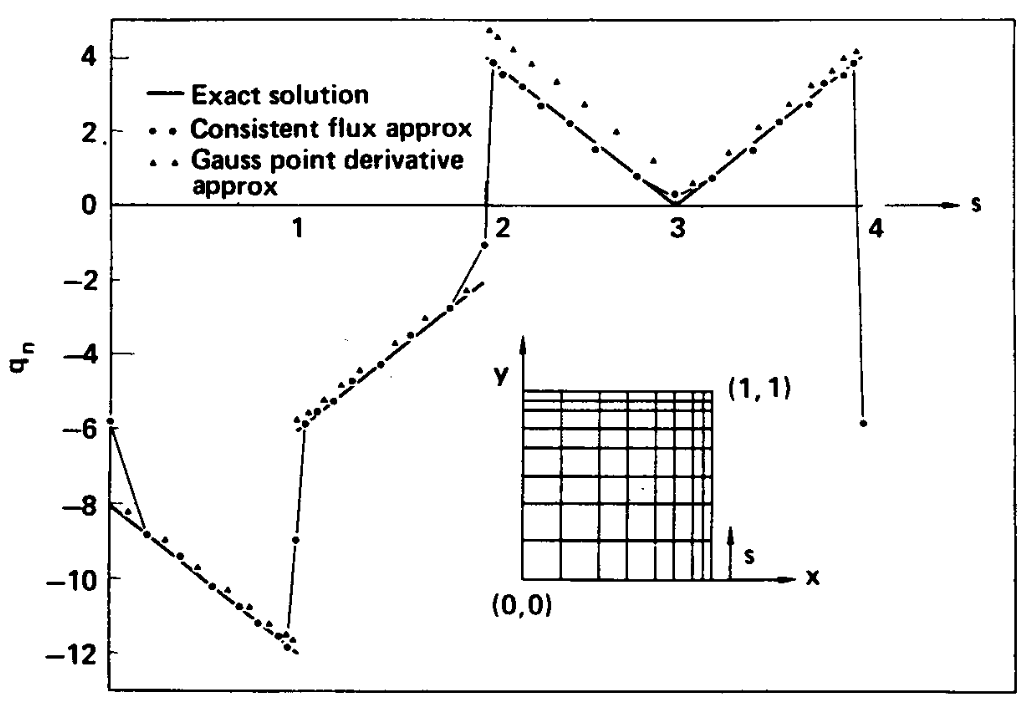
\includegraphics[width=7.5cm]{python_codes/fieldstone_173/images/grls87a}\\
{\captionfont Rather annoyingly the figure of the paper is poorly digitized 
to the point that it is somewhat dificult to distinguish between dots and triangles data points.}
\end{center}

These observations motivate the following section.
Also, this problem is not new and we read in \textcite{mizu86} (1986):
\begin{displayquote}
Most finite element schemes for thermal problems estimate boundary heat flux directly from the
derivative of the finite element solution. The boundary flux calculated by this approach is typically
inaccurate and does not guarantee a global heat balance.
\end{displayquote}

%==============================================================================
\section*{Computing the boundary heat flux}

In \textcite{mizu86} (1986) we find\footnote{I have replaced $\phi$ by $T$ and 
the source term $f$ by $S$.}
\[
\sum_{k \in \Gamma_g} \int_{\Gamma_g} \bN_i \bN_k d\Gamma \; 
\left(
\frac{\partial T}{\partial n}
\right)_k
=
\int_\Omega \vec\nabla \bN_i \cdot \vec\nabla T^h \; d\Omega
- \int_\Omega \bN_i S \; d\Omega
\qquad
i \in \Gamma_g
\]
where $T^h$ is the computed temperature and $\Gamma_g$ is the part of the 
boundary where Dirichelt boundary conditions are imposed.








